%%%%%%%%%%%%%%%%%%%%%%%%%%%%%%%%%%%%%%%%%
% Short Sectioned Assignment
% LaTeX Template
% Version 1.0 (5/5/12)
%
% This template has been downloaded from:
% http://www.LaTeXTemplates.com
%
% Original author:
% Frits Wenneker (http://www.howtotex.com)
%
% License:
% CC BY-NC-SA 3.0 (http://creativecommons.org/licenses/by-nc-sa/3.0/)
%
%%%%%%%%%%%%%%%%%%%%%%%%%%%%%%%%%%%%%%%%%

%----------------------------------------------------------------------------------------
%	PACKAGES AND OTHER DOCUMENT CONFIGURATIONS
%----------------------------------------------------------------------------------------

\documentclass[paper=a4, fontsize=11pt]{scrartcl} % A4 paper and 11pt font size
\usepackage{float}
\usepackage{listings}
\usepackage{color}

\definecolor{dkgreen}{rgb}{0,0.6,0}
\definecolor{gray}{rgb}{0.5,0.5,0.5}
\definecolor{mauve}{rgb}{0.58,0,0.82}

\lstset{frame=tb,
  language=MATLAB,
  aboveskip=3mm,
  belowskip=3mm,
  showstringspaces=false,
  columns=flexible,
  basicstyle={\small\ttfamily},
  numbers=none,
  numberstyle=\tiny\color{gray},
  keywordstyle=\color{blue},
  commentstyle=\color{dkgreen},
  stringstyle=\color{mauve},
  breaklines=true,
  breakatwhitespace=true,
  tabsize=3
}

\usepackage{CJKutf8} % chinese support
\usepackage{graphicx}

\usepackage[T1]{fontenc} % Use 8-bit encoding that has 256 glyphs
\usepackage{fourier} % Use the Adobe Utopia font for the document - comment this line to return to the LaTeX default
\usepackage[english]{babel} % English language/hyphenation
\usepackage{amsmath,amsfonts,amsthm} % Math packages

\usepackage{lipsum} % Used for inserting dummy 'Lorem ipsum' text into the template

\usepackage{sectsty} % Allows customizing section commands
\allsectionsfont{\centering \normalfont\scshape} % Make all sections centered, the default font and small caps

\usepackage{fancyhdr} % Custom headers and footers
\pagestyle{fancyplain} % Makes all pages in the document conform to the custom headers and footers
\fancyhead{} % No page header - if you want one, create it in the same way as the footers below
\fancyfoot[L]{} % Empty left footer
\fancyfoot[C]{} % Empty center footer
\fancyfoot[R]{\thepage} % Page numbering for right footer
\renewcommand{\headrulewidth}{0pt} % Remove header underlines
\renewcommand{\footrulewidth}{0pt} % Remove footer underlines
\setlength{\headheight}{13.6pt} % Customize the height of the header

\numberwithin{equation}{section} % Number equations within sections (i.e. 1.1, 1.2, 2.1, 2.2 instead of 1, 2, 3, 4)
\numberwithin{figure}{section} % Number figures within sections (i.e. 1.1, 1.2, 2.1, 2.2 instead of 1, 2, 3, 4)
\numberwithin{table}{section} % Number tables within sections (i.e. 1.1, 1.2, 2.1, 2.2 instead of 1, 2, 3, 4)

\setlength\parindent{0pt} % Removes all indentation from paragraphs - comment this line for an assignment with lots of text

%----------------------------------------------------------------------------------------
%	TITLE SECTION
%----------------------------------------------------------------------------------------

\newcommand{\horrule}[1]{\rule{\linewidth}{#1}} % Create horizontal rule command with 1 argument of height

\title{
\normalfont \normalsize 
\textsc{计算物理学15春季} \\ [25pt] % Your university, school and/or department name(s)
\horrule{0.5pt} \\[0.4cm] % Thin top horizontal rule
\huge 计算物理学作业解题报告 \\ % The assignment title
\horrule{2pt} \\[0.5cm] % Thick bottom horizontal rule
}

\author{霍浩岩} % Your name

\date{\normalsize\today} % Today's date or a custom date

\begin{document}
\begin{CJK*}{UTF8}{gbsn}

\maketitle % Print the title

%----------------------------------------------------------------------------------------
%	PROBLEM 1
%----------------------------------------------------------------------------------------

\section{表针三等分表盘问题}

\subsection{评估函数的选取}
这里使用的评估函数和题目中的有所不同。规定时针、分针、秒针的转角分别为$h$、$m$、$s$,它们的取值范围不限于$[0,2\pi)$,而是从零时刻开始到12小时结束之间连续变化的,也就是说,$h\in [0,2\pi]$,$m\in [0,24\pi]$,$s\in [0,1440\pi]$。\\\\
评估函数首先将这三个转角模掉$2\pi$,然后将它们按从小到大排列成$\theta_1$,$\theta_2$,$\theta_3$,可以定义评估函数:

\begin{align}
[f(h,m,s)]^2 
&= (\theta_2-\theta_1-\frac{2\pi}{3})^2 + (\theta_3-\theta_2-\frac{2\pi}{3})^2 + (\theta_1-\theta_3-\frac{4\pi}{3})^2 \\
\theta_1 &= min(h,m,s) \\
\theta_2 &= mid(h,m,s) \\
\theta_3 &= max(h,m,s)
\end{align}

\lstset{language=MATLAB}
\begin{lstlisting}
function cost = cost_function(h,m,s)
  h = mod(h,2*pi);
  m = mod(m,2*pi);
  s = mod(s,2*pi);

  sorted = sort([h(:) m(:) s(:)], 2);
  t1 = sorted(:,1); t2 = sorted(:,2); t3 = sorted(:,3);

  cost = (t2-t1-2*pi/3).^2 + (t3-t2-2*pi/3).^2 + (t1-t3-4*pi/3).^2;
end

function cost=cost_function_t(t)
  cost = cost_function(t/12*2*pi, t*2*pi, t*60*2*pi);
end
\end{lstlisting}

为了首先得到一个比较直观的评估函数变化的图景,可以将这个函数从零时刻到12小时整个区间内的图像画出来。

\lstset{language=MATLAB}
\begin{lstlisting}
t = [0:1/3600*2:12];
y = cost_function(t/12*2*pi,t*2*pi,t*60*2*pi);
plot(t,y);
xlabel('time/hour');
ylabel('cost function');
\end{lstlisting}


\begin{figure}[ht!]
\centering
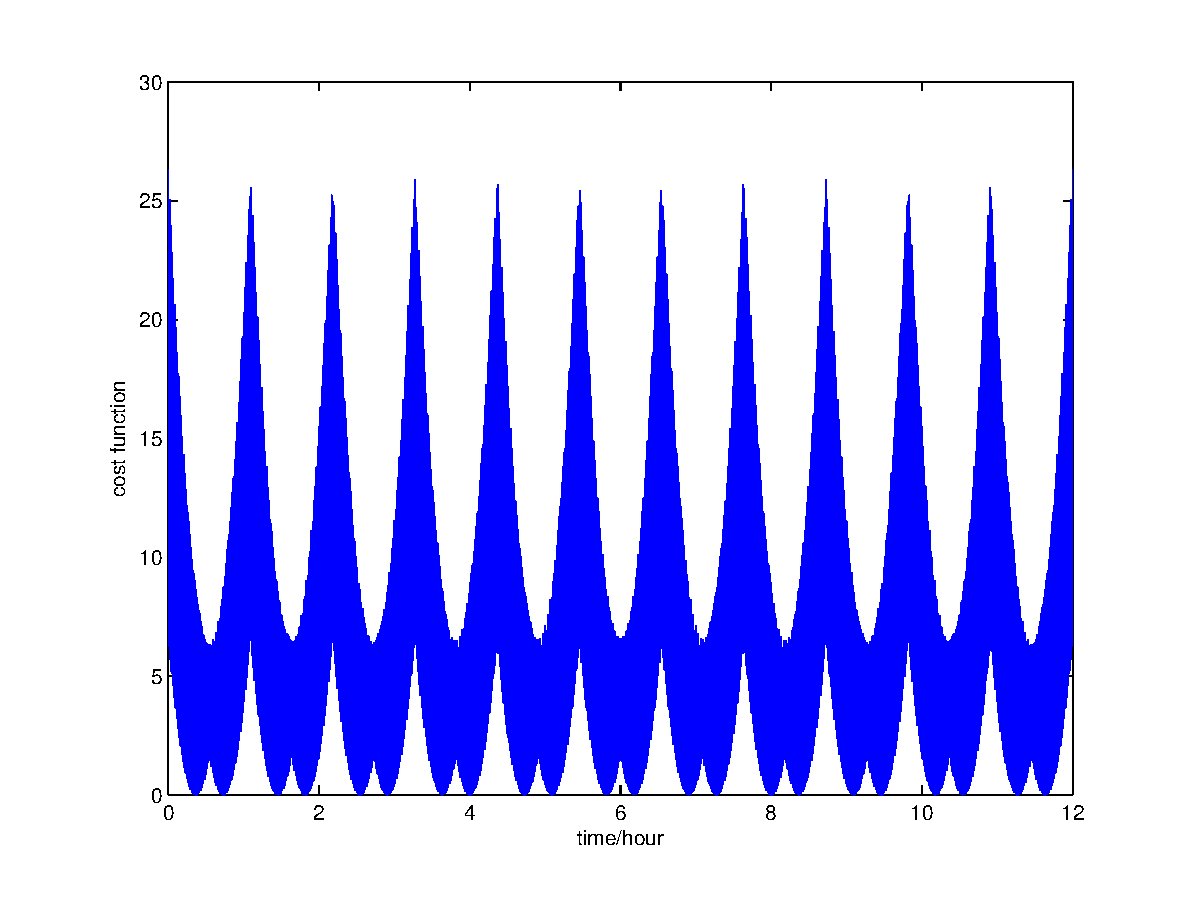
\includegraphics[width=90mm]{problem1_cost_function.eps}
\caption{评估函数在整个时间区间内的变化}
\end{figure}

\subsection{函数极小值的寻找}
从上图中可以看到,评估函数具有22个极小值,然而它们的大小以及它们是否为零还需要进一步的考察。在每一个近似极小值附近使用MATLAB的fminbnd函数寻找极小值的精确值,然后将这些精确值排序:

\lstset{language=MATLAB}
\begin{lstlisting}
mt = sortrows([t(:) y(:)],2);
                               % search minimum in +/-1 minute
deltaT = 1/3600*60;
final_result = [];
for j=1:22
  x = fminbnd(@cost_function_t, mt(j,1)-deltaT, mt(j,1)+deltaT);
  final_result = [final_result;x cost_function_t(x)];
end
final_result = sortrows(final_result, 2);
x1 = final_result(1,1); x2=final_result(2,1);
y1 = final_result(1,2); y2=final_result(2,2);

display('using fminbnd@MATLAB to find the actual solution as:');
display(sprintf('%.10f %.10f', x1, x2));
display('cost function at solution is:');
display(sprintf('%.10f %.10f', y1, y2));
\end{lstlisting}
求解得到,当时间等于$t=2.90960 h$、$t=9.09034 h$的时候,评估函数到达极小$0.000012922$。这就是我们要找的最接近三等分表盘的时刻,对应的时分秒针角度分别为:$$(87.2880^{\circ},327.4562^{\circ},207.3701^{\circ})$$ $$(272.7120^{\circ}, 32.5438^{\circ},152.6299^{\circ})$$

\subsection{求解程序}
\lstset{language=MATLAB}
\begin{lstlisting}
%%%%%%%%%%%%%%%%%%%%
% call me!
%%%%%%%%%%%%%%%%%%%%
function clock3
  t = [0:1/3600*2:12];
  y = cost_function_t(t);

  plot(t,y);
  xlabel('time/hour');
  ylabel('cost function');

  mt = sortrows([t(:) y(:)],2);

                                % search minimum in +/-1 minute
  deltaT = 1/3600*60;
  final_result = [];
  for j=1:22
    x = fminbnd(@cost_function_t, mt(j,1)-deltaT, mt(j,1)+deltaT);
    final_result = [final_result;x cost_function_t(x)];
  end
  final_result = sortrows(final_result, 2);
  x1 = final_result(1,1); x2=final_result(2,1);
  y1 = final_result(1,2); y2=final_result(2,2);

  display('using fminbnd@MATLAB to find the actual solution as:');
  display(sprintf('%.10f %.10f', x1, x2));
  display('cost function at solution is:');
  display(sprintf('%.10f %.10f', y1, y2));

  function cost=cost_function_t(t)
    cost = cost_function(t/12*2*pi, t*2*pi, t*60*2*pi);
  end

  function cost = cost_function(h,m,s)
    h = mod(h,2*pi);
    m = mod(m,2*pi);
    s = mod(s,2*pi);

    sorted = sort([h(:) m(:) s(:)], 2);
    t1 = sorted(:,1); t2 = sorted(:,2); t3 = sorted(:,3);

    cost = (t2-t1-2*pi/3).^2 + (t3-t2-2*pi/3).^2 + (t1-t3+4*pi/3).^2;
  end
end

\end{lstlisting}

\pagebreak

\section{含有Zeta函数的方程求解}

\subsection{无穷求和}
\begin{align}
\begin{split}
\mathcal{Z}_{00}(1;q^2) &= \sum_\mathbf{n} \frac{e^{q^2-\mathbf{n}^2}}{\sqrt{4\pi}(\mathbf{n}^2-q^2)}-\pi +\frac{\pi}{2}\int_0^1t^{-3/2}(e^{tq^2}-1)dt \\\\ &+ \sqrt{\frac{\pi}{4}} \int_0^1 t^{-3/2}(\sum_{\mathbf{n}\neq 0} e^{tq^2}e^{-(\pi^2/t)\mathbf{n}^2})dt
\end{split}
\end{align}
现在需要估计在指定精度下上式中的求和项应该保留多少项。在这之前需要对整个计算式的量级有一个大概的估计,然而在没有计算之前这是比较困难的,不妨就先假设整个计算式的量级为$10^0$。

在第一个求和计算中,考虑到$q\in (0,3)$,$\mathbf{n}^2$的前几项有可能与$q$十分接近,所以前几项有可能分母非常小,必须保留。从$n^2>9$开始,分母总是一个大于1的数,而分子则随着$\mathbf{n}$的增加迅速衰减,做估计:
\begin{equation}
\frac{e^{q^2-\mathbf{n}^2}}{\mathbf{n}^2-q^2} \leq e^{q^2-\mathbf{n}^2} \leq 10^{-6}
\end{equation}
得到$\mathbf{n}^2\geq q^2+12 \approx 15$,也就是说,我们的有限求和需要取那些$\mathbf{n}^2 \leq 15$的三维整数,将所有三维整数按照他们的模方大小排序,并把三个数绝对值集合相同的三维整数算作一个求和项,需要求和的整数就是:$
\mathbf{n}^2 = (0,0,0),$ $ (0,0,1),(0,1,1),(1,1,1)$ $,(0,0,2),(0,1,2),
(1,1,2),$ $(0,2,2),$ $(0,0,3),(1,2,2),(0,1,3),(1,1,3),$ $(2,2,2),(0,2,3),(1,2,3)
$
,共有15项。
\\\\
要求精度$10^{-12}$时,用同样的办法估计出求和项需要到第40项,具体的三维整数就不在这里写出了。另外,保守起见,可以将这个求和项略微增加一些。
\\\\
对于后一项求和,由于$\pi^2/t > 1$,它的每项的衰减速率比第一个求和还要快,因此15项也能达到很高的精度。
\\\\
在$q$较小(例如$q^2<0.001$)的时候,整个计算式呈现发散,这是因为第一个求和的第一项$\frac{e^{q^2}}{-q^2}$发散,于是可以估计出在$q^2$小的时候:
\begin{equation}
\mathcal{Z}_{00}(1;q^2) \approx -\frac{1}{\sqrt{4\pi}q^2}
\end{equation}
\\\\\\\\
\subsection{散射相移方程求解}
在这里我们仍然需要估计整个Zeta函数的值的量级。考虑带求解的方程:
\begin{equation}
\pi^{3/2}(\frac{1}{A_0}+\frac{R_0}{2}q^2) = \mathcal{Z}_{00}(1;q^2)
\end{equation}
可以看到方程左边是大于1的,因此我们上面第一小题中估计的量级合适。
\\\\
写出整个Zeta函数的表达式,然后就可以求解这个非线性方程了,MATLAB中有求解非线性方程的函数fsolve[1],使用了所谓的“置信域”算法(这是默认的算法,还可以选择“trust-region-reflective”和“levenberg-marquardt”算法,默认的“trust-region-dogleg”已经足够求出方程的解)。
\\\\
求解的结果是:
\begin{equation}
q^2 = 0.794516
\end{equation}
程序如下:

\lstset{language=MATLAB}
\begin{lstlisting}
%%%%%%%%%%%%%%%%%%%%
% call me!
%%%%%%%%%%%%%%%%%%%%
function main()
  q2 = 0.90;

  [x, fval, exitflag] = fsolve(@tosolve, q2);
  display(sprintf('problem solved, flag=%d, x=%.6f, fval=%.12f', exitflag, x, fval));
end

function total = tosolve(q2)
  total = zeta00(q2)/(pi^(3/2)) - 1 - 0.25*q2;
end

function total = zeta00(q2)
  total = zeta00_part_1(q2) + zeta00_part_2(q2) + zeta00_part_3(q2) + zeta00_part_4(q2);
end

function total = zeta00_part_4(q2)
  function s = innersum(x)
    s = zeros(size(x,1), size(x,2));
    tdints = threed_integers();
    for j=2:size(tdints,1)
      n_squared = sum((tdints(j,1:3)).^2);
      s = s + exp(x*q2).*exp(-1./x*n_squared*(pi^2)) * tdints(j,4);
    end
    s = x.^(-1.5).*s;
  end
  fun = @(x) innersum(x);
  total = integral(fun, 0, 1)*sqrt(pi/4);
end

function total = zeta00_part_3(q2)
  fun = @(x) x.^(-1.5).*(exp(x.*q2)-1);
  total = integral(fun, 0, 1) * pi / 2;
end

function total = zeta00_part_2(q2)
  total = -pi;
end

function total = zeta00_part_1(q2)
  total = 0;

  tdints = threed_integers();
  for j=1:size(tdints, 1)
    n_squared = sum((tdints(j,1:3)).^2);
    total = total + exp(q2-n_squared) / (n_squared-q2) * tdints(j,4);
  end

  total = total /sqrt(4*pi);
end

function result = threed_integers()
  tbl = [0 0 0 1;...
         0 0 1 6;...
         0 1 1 12;...
         1 1 1 8;...
         0 0 2 6;...
         0 1 2 24;...
         1 1 2 24;...
         0 2 2 12;...
         0 0 3 6;...
         1 2 2 24;...
         0 1 3 24;...
         1 1 3 24;...
         2 2 2 8;...
         0 2 3 24;...
         1 2 3 48;];

  result = tbl;
end

\end{lstlisting}



\pagebreak
\section{关联函数的拟合与数据分析}
\subsection{样本平均值来估计函数 $C(t)$ 的中心值}
首先根据题目的要求,读入数据并构建对称化的函数值:

\lstset{language=MATLAB}
\begin{lstlisting}
data = dlmread('pion-correlation-function.dat', '', 1);

symmetric_data = cell(250,1);
for i=1:250
  symmetric_data{i} = symmetric_piece(data((i-1)*64+1:i*64,:));
end

function result = symmetric_piece(piece)
  result = zeros(33, 2);

  for i=0:32
    if i==0
      result(i+1,:) = piece(1,2:3);
    else
      result(i+1,:) = 0.5*(piece(i+1,2:3) + piece(64-i+1,2:3));
    end
  end
end
\end{lstlisting}
读入的数据中包含实部和虚部,可以看到实部在量级上远远大于虚部,猜想到虚部数据将由于远小于实部的误差而可以舍去。用下面的代码计算实部和虚部的误差及其均值:

\lstset{language=MATLAB}
\begin{lstlisting}
%%%%%%%%%%%%%%%%%%%%
% problem a)
%%%%%%%%%%%%%%%%%%%%
data_real = zeros(250, 33);
data_image = zeros(250, 33);
for i=1:250
  data_real(i,:) = symmetric_data{i}(:,1);
  data_image(i,:) = symmetric_data{i}(:,2);
end
avg_real = mean(data_real); avg_image = mean(data_image);
delta_real = sqrt(var(data_real)/250); delta_image = sqrt(var(data_image)/250);

figure;
plot(delta_real ./ avg_real);

\end{lstlisting}
分析计算结果,标记虚部均值的数组\textit{avg\_image}量级是$10^{-16}$,而标记实部误差的数组\textit{delta\_real}量级是1,所以可以放心的略去虚部,而只考虑实部。
\\\\
相对误差$\Delta C(t) / \overline{C}(t)$的图像如下:


\begin{figure}[H]
\centering
\includegraphics[width=140mm]{problem3_a_1.eps}
\caption{相对误差$\Delta C(t) / \overline{C}(t)$}
\end{figure}

使用线性函数来拟合这个图线:
\lstset{language=MATLAB}
\begin{lstlisting}
relative_delta = delta_real ./ avg_real;
plot([1:33],relative_delta,'.');

coefficients = polyfit([1:33], relative_delta, 1);
a = coefficients(1);
b = coefficients(2);

hold on;
plot([1:33], b+a*[1:33]);
\end{lstlisting}
得到的相对误差随时间变化关系为:
\begin{equation}
\Delta C(t) / \overline{C}(t) = (0.155+0.0114 t) \%
\end{equation}
\begin{figure}[H]
\centering
\includegraphics[width=140mm]{problem3_a_2.eps}
\caption{相对误差$\Delta C(t) / \overline{C}(t)$}
\end{figure}

\subsection{Jackknife估计$m_{eff}(t)$}
为了估计$m_{eff}(t)$,使用jackknife方法进行重抽样操作。MATLAB中已经为我们准备好了jackknife重抽样操作函数,因此就不必手动写重抽样的循环代码(需注意题目中时间下标恰好与MATLAB中的下标差1):
\lstset{language=MATLAB}
\begin{lstlisting}
%%%%%%%%%%%%%%%%%%%%
% problem b) jackknife
%%%%%%%%%%%%%%%%%%%%
resampled_avgs = jackknife(@mean, data_real, 1);
resampled_meff_t = log(resampled_avgs(:,1:32) ./ resampled_avgs(:,2:33));
resampled_length = size(resampled_meff_t, 1);
meff_t = mean(resampled_meff_t);
delta_meff_t = sqrt((resampled_length-1)^2/resampled_length*var(resampled_meff_t));
figure;
plot([0:31], delta_meff_t, '.');
figure;
errorbar([0:31], meff_t, delta_meff_t, '.k');
\end{lstlisting}
上面的代码画出了整个时间片的有效质量结果和它们的误差,如下(误差棒太小以至于看不清楚了):
\begin{figure}[H]
\centering
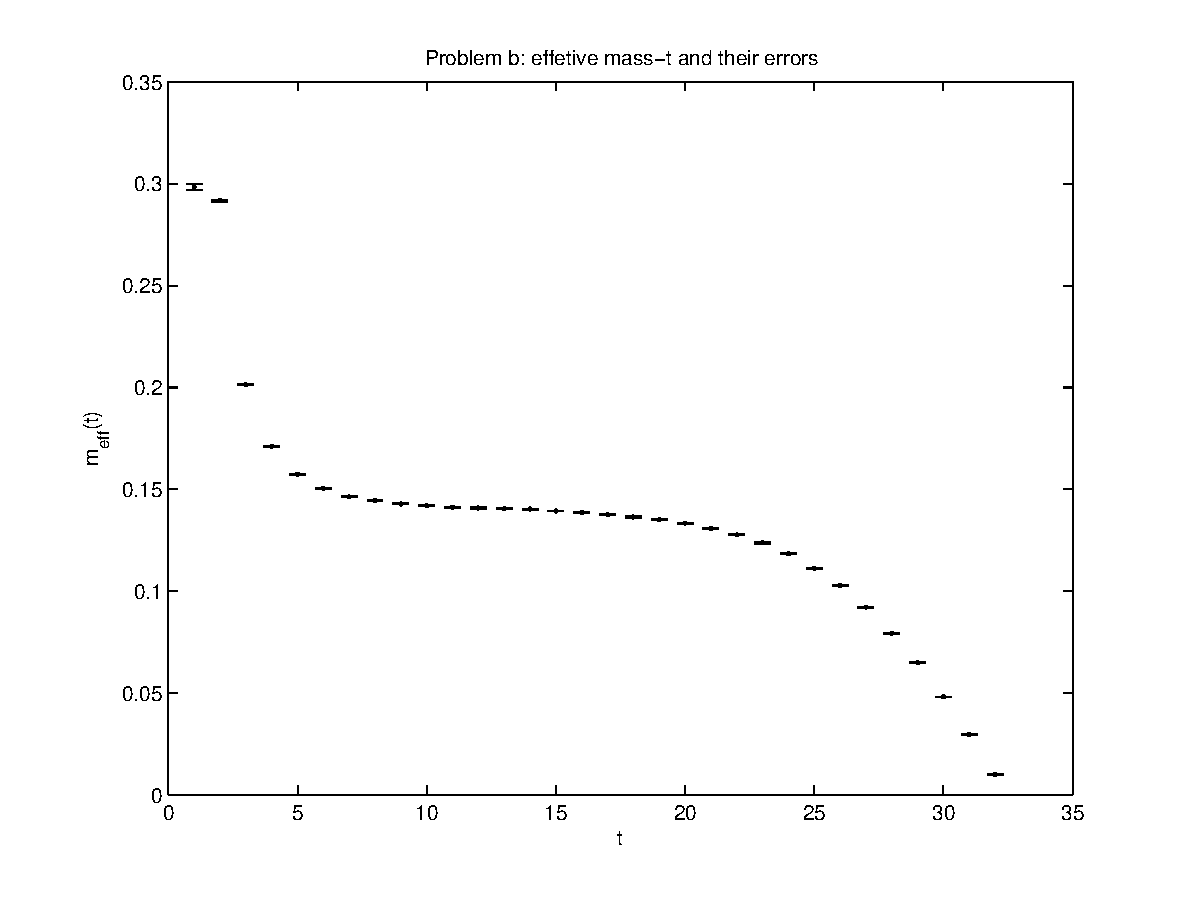
\includegraphics[width=150mm]{problem3_b_1.eps}
\caption{整个时间片上的$m_{eff}(t)$和误差}
\end{figure}
发现在时间片中间,有一段“平台区”,这也是我们接下来需要拟合的数据区域。单独将每个时间点的误差画出:
\begin{figure}[H]
\centering
\includegraphics[width=150mm]{problem3_b_2.eps}
\caption{整个时间片上的$\Delta m_{eff}(t)$}
\end{figure}
\subsection{$\chi^2$拟合}
希望拟合函数
\begin{equation}
f_i(m_\pi) = f(z_i;m_\pi) = m_\pi
\end{equation}
使得$\chi^2$最小:
\begin{equation}
\chi^2 = \sum_{t=t_{min}}^{t=t_{max}} (\frac{m_{eff}(t)-f_t(m_\pi)}{\Delta m_{eff}(t)})^2
\end{equation}
假设有$n$个时间节点,那么需要构建一个$n \times 1$设计矩阵,满足:
\begin{equation}
\frac{f_t(x)}{\Delta m_{eff}(t)} = A_{t1}m_\pi
\end{equation}
由此可以得到设计矩阵的矩阵元:
\begin{equation}
A_{t1} = \frac{1}{\Delta m_{eff}(t)}
\end{equation}
利用下式进行线性最小$\chi^2$拟合:
\begin{equation}
(A^TA)m_\pi = A^T \widetilde{y}
\end{equation}
其中,$\widetilde{y} = m_{eff}(t)/ \Delta m_{eff}(t)$。

为了确定拟合的开始时间点和结束时间点,需要对上面求出的$m_{eff}(t)$进行扫描。通过一段连续的时间片(至少有4个点),拟合出$m_\pi$和它的误差。其中$m_\pi$的误差计算方法如下:
\begin{equation}
\Delta \chi^2 = \Delta m_\pi^2 (A^T A)
\end{equation}
其中,$\Delta \chi^2$是选取的一定置信度水平的$\Delta \chi^2$的数值,这里我们选择$99\%$置信水平,相应的值可以通过MATLAB自带的$chi2cdf$函数计算出来。

下面的程序中,chi2\_best\_fit对整个时间片扫面,试图找到$\chi^2$最小即最优的拟合区间。每次拟合由chi2\_fit函数完成。
\lstset{language=MATLAB}
\begin{lstlisting}
%%%%%%%%%%%%%%%%%%%%
% problem c)
%%%%%%%%%%%%%%%%%%%%
[meff, dmeff, chi2, pvalue, tstart, tend] = chi2_best_fit(meff_t, delta_meff_t, 4);
display(sprintf('fitting result: meff: %f, dmeff: %f, chi2: %f, pvalue: %f, tstart: %d, tend: %d', meff, dmeff, chi2, pvalue, tstart-1, tend-1));
hold on;
line([5 30], [meff meff]);
a = axis; miny = a(3); maxy = a(4);
line([tstart tstart], [miny+0.15*(maxy-miny) maxy-0.15*(maxy-miny)]);
line([tend tend], [miny+0.15*(maxy-miny) maxy-0.15*(maxy-miny)]);

function [result, dresult, chi_squared, pvalue, tstart, tend] = chi2_best_fit(input_seq, dinput_seq, pt_lbound)
  input_seq = input_seq(:);
  dinput_seq = dinput_seq(:);
  time_start = 1;
  time_end = size(input_seq,1);
  
  best_fit = [0 9999999 9999 -1 -1];
  for a=time_start:time_end
    for b=pt_lbound-1:50
      tstart = a;
      tend = tstart+b;
      if tend > time_end
        break
      end
      [mpi, dmpi, chi_2] = chi2_fit(input_seq(tstart:tend), dinput_seq(tstart:tend));
      if (dmpi<best_fit(2)&&chi_2<best_fit(3)) || chi_2 < best_fit(3)
        best_fit = [mpi dmpi chi_2 tstart tend];
      end
    end
  end
  result = best_fit(1);
  dresult = best_fit(2);
  chi_squared = best_fit(3);
  tstart = best_fit(4);
  tend = best_fit(5);
  pvalue = chi2cdf(chi_squared, tend-tstart);
end

function [x,dx,chi_2] = chi2_fit(input, dinput)
  input = input(:);
  dinput = dinput(:);
  N = size(input,1);

  A = 1./dinput;
  y = input ./ dinput;
  x = transpose(A)*y/(transpose(A)*A);
  chi_2 = sum((y-A*x).^2);
  dx = sqrt(chi2inv(chi2cdf(9,1), N)/(transpose(A)*A));
end
\end{lstlisting}
经过扫描,程序给出最优的拟合区域是$[10,13]$(自由度为3),相应的拟合结果是$m_{eff}\pm \Delta m_{eff}=0.14074\pm0.00048$,$\chi^2=9.649599$,$pvalue=0.978208$。
\begin{figure}[H]
\centering
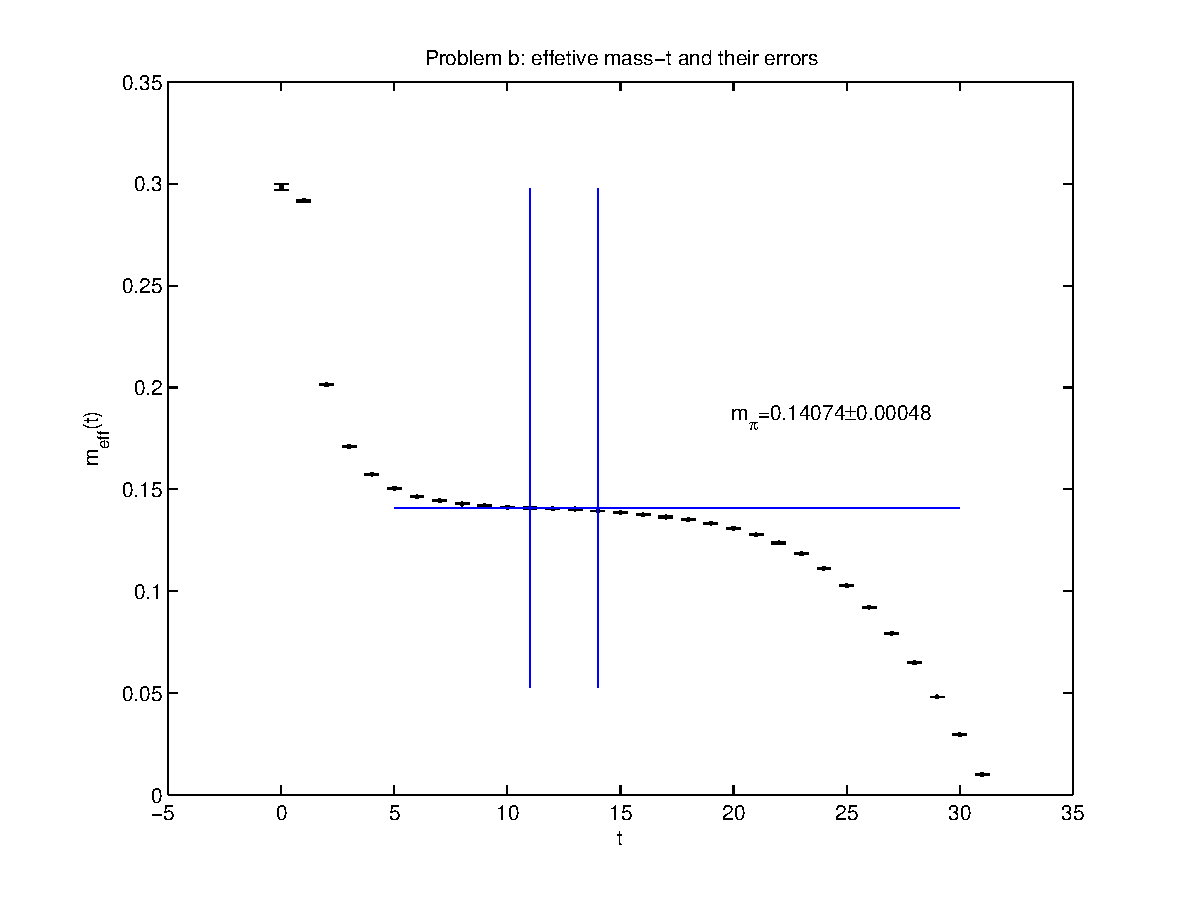
\includegraphics[width=150mm]{problem3_c_1.eps}
\caption{单变量线性拟合结果和原来的数据点}
\end{figure}

\subsection{构建新的 ratio 拟合}
按照题目的公式给出新的ratio定义,绘制出时间区间内新ratio的变化趋势:
\begin{figure}[H]
\centering
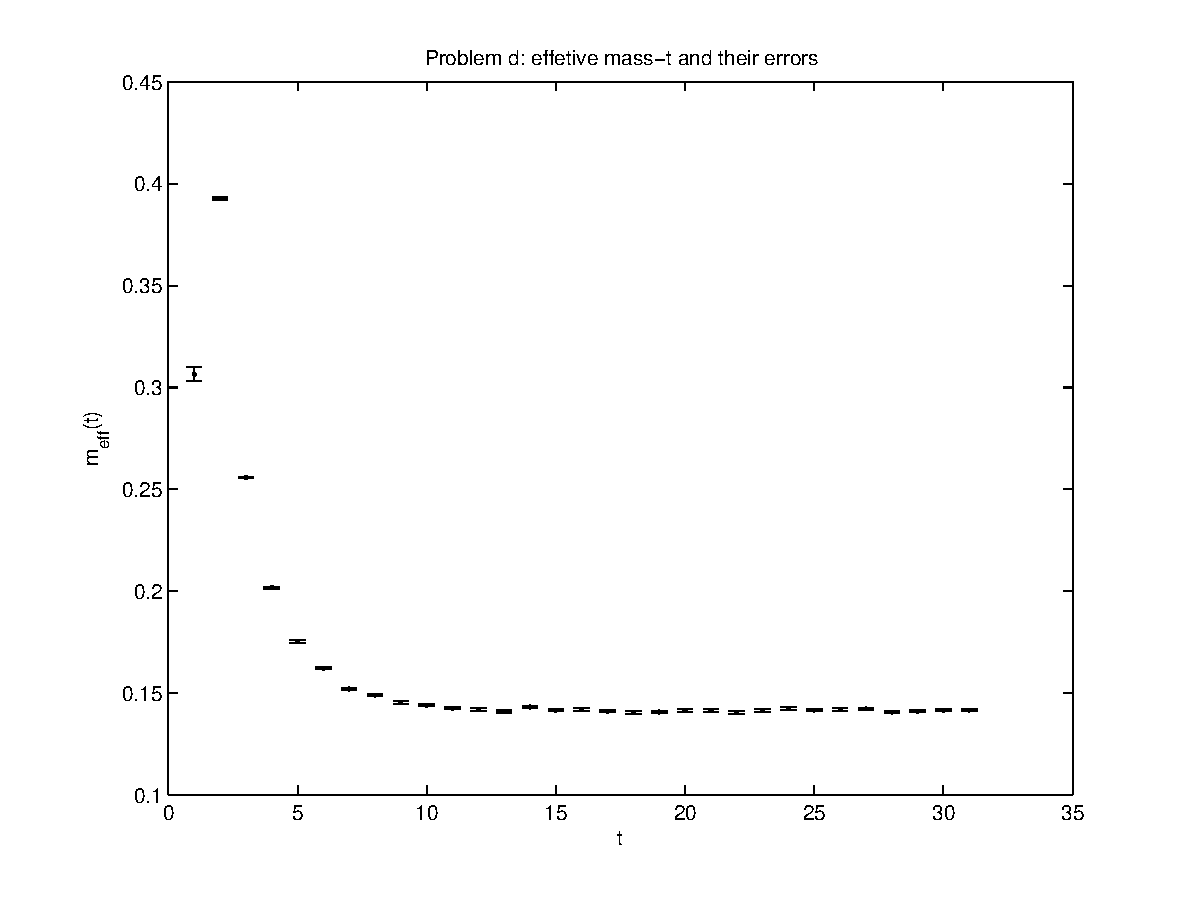
\includegraphics[width=140mm]{problem3_d_1.eps}
\caption{整个时间片上的新$m_{eff}(t)$和误差}
\end{figure}
这次数据一直到平台区域末端都可以比较好的拟合,再次使用$\chi^2$拟合:
\lstset{language=MATLAB}
\begin{lstlisting}
%%%%%%%%%%%%%%%%%%%%
% problem d)
%%%%%%%%%%%%%%%%%%%%
resampled_avgs_2 = jackknife(@mean, data_real, 1);
resampled_meff_t_2 = acosh((resampled_avgs_2(:,1:31) + (resampled_avgs_2(:,3:33))) ./ 2 ./ resampled_avgs_2(:,2:32));
resampled_length_2 = size(resampled_meff_t_2, 1);
meff_t_2 = mean(resampled_meff_t_2);
delta_meff_t_2 = sqrt((resampled_length_2-1)^2/resampled_length_2*var(resampled_meff_t_2));
figure;
errorbar([1:31], meff_t_2, delta_meff_t_2, '.k');
xlabel('t');
ylabel('m_{eff}(t)');
title('Problem d: effetive mass-t and their errors');

[meff_2, dmeff_2, chi2_2, pvalue_2, tstart_2, tend_2] = chi2_best_fit(meff_t_2, delta_meff_t_2, 4);
display(sprintf('fitting result: meff: %f, dmeff: %f, chi2: %f, pvalue: %f, tstart: %d, tend: %d', meff_2, dmeff_2, chi2_2, pvalue_2, tstart_2, tend_2));
hold on;
line([5 30], [meff meff]);
a = axis; miny = a(3); maxy = a(4);
line([tstart_2 tstart_2], [miny+0.05*(maxy-miny) miny+0.3*(maxy-miny)]);
line([tend_2 tend_2], [miny+0.05*(maxy-miny) miny+0.3*(maxy-miny)]);
\end{lstlisting}
新的最优拟合区域是$[20,23]$(自由度为3),相应的拟合结果是$m_{eff}\pm \Delta m_{eff}=0.1412\pm0.0013$,$\chi^2=1.051026$,$pvalue=0.211092$。和上面的拟合相比,$pvalue$有所下降,结果的置信度提高了,但是$m_\pi$结果的不确定度变大了。
\\\\
这个结果不难理解:在第一次拟合中,中间尽管有一段平台区域,但多多少少会受到前面和后面非平台区域的影响,数据点的分布并不好,拟合结果$\chi^2$较大就说明了这一点;而第二次拟合中,平台区域从中间一直延伸到末端,可以预期数据的分布较好,$\chi^2$较小验证了这一点,但是因为后面的数据信噪比变差,拟合出的参数(即$m_\pi$)误差也就随之变大了。

\subsection{相关系数矩阵}
bootstrap就是从$N=250$个组态中随机选取250个组态计算统计量,共计算$N_B=1000$次。然后计算它们的统计量,再对统计量计算均值和误差。然而MATLAB已经为我们提供了方便的bootstrp函数实现这个操作:
\lstset{language=MATLAB}
\begin{lstlisting}
[bootstat, bootsam] = bootstrp(1000, @cov, data_real);
cov_mean = mean(bootstat);
\end{lstlisting}
cov是MATLAB中计算数据协方差矩阵的函数。执行bootstrp函数之后,bootstat就包含了一个$1000\times (33\times33)$的矩阵,每一行都是一个bootstrap sample计算出的协方差矩阵(当然已经将矩阵压缩成行向量存储),bootsam的每一行包含了随机选中的组态下标数(然而这里并不会用到)。根据这些组态计算出的协方差矩阵,我们求出协方差矩阵的均值和上下界:
\begin{lstlisting}
cov_mean = mean(bootstat);
cov_low_bound = zeros(1, size(cov_mean,2));
cov_top_bound = zeros(1, size(cov_mean,2));
for j=1:size(cov_mean,2)
  sorted_cov = sortrows(bootstat(:,j),1);
  cov_low_bound(j) = sorted_cov(160);
  cov_top_bound(j) = sorted_cov(840);
end
N = size(data_real,2);
cov_mean = reshape(cov_mean, [N,N]);
cov_low_bound = reshape(cov_low_bound, [N N]);
cov_top_bound = reshape(cov_top_bound, [N N]);
cov_delta = (cov_top_bound - cov_low_bound)/2;
\end{lstlisting}
此时cov\_mean和cov\_delta就是协方差矩阵的均值和误差了。还可以从cov\_low\_bound和cov\_top\_bound中确定协方差矩阵的上界和下界。

为了对这个矩阵有直观的了解,首先来看矩阵元素的散点图:
\begin{figure}[H]
\centering
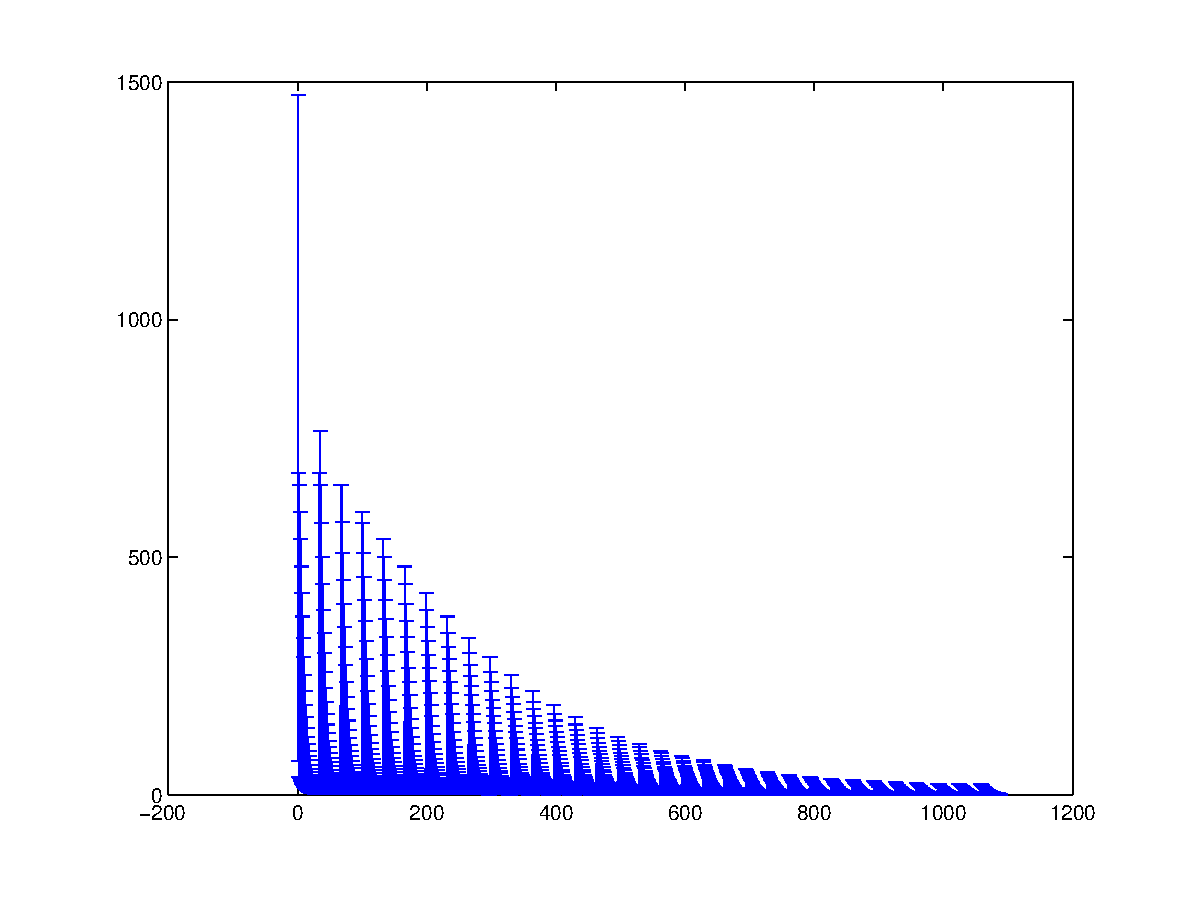
\includegraphics[width=140mm]{problem3_e_1.eps}
\caption{协方差矩阵压缩成行向量}
\end{figure}
可以发现矩阵的上部关联比较明显,为了进一步观察协方差矩阵的特征,画出均值的二维图:
\begin{figure}[H]
\centering
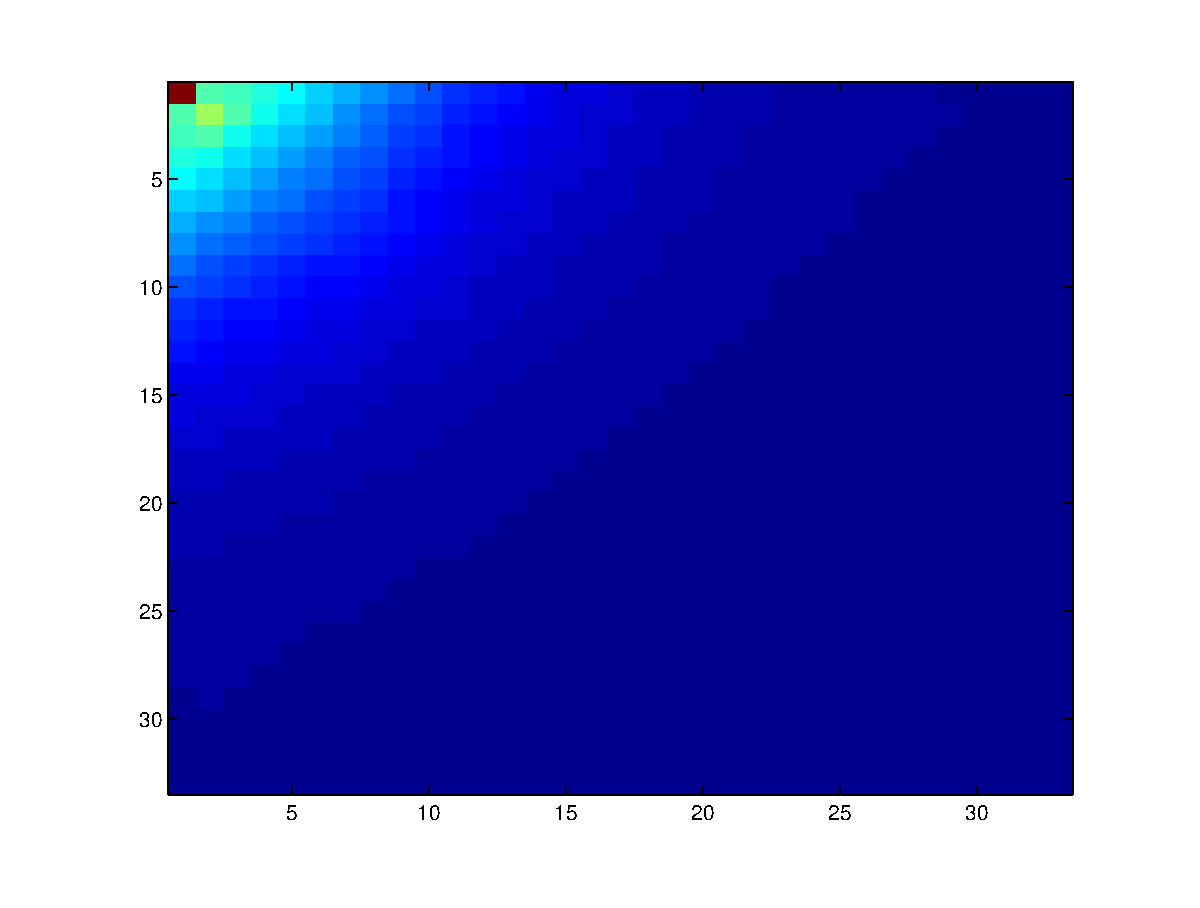
\includegraphics[width=140mm]{problem3_e_2.eps}
\caption{协方差矩阵的二维图}
\end{figure}
这一次就能更清楚的看到时间片前部分的相关度要明显大一些。
\\\\
同样的方法可以计算相关矩阵(MATLAB中计算相关矩阵的函数corrcoef):
\begin{lstlisting}
[bootstat, bootsam] = bootstrp(1000, @corrcoef, data_real);
corrcoef_mean = mean(bootstat);
corrcoef_low_bound = zeros(1, size(corrcoef_mean,2));
corrcoef_top_bound = zeros(1, size(corrcoef_mean,2));
for j=1:size(corrcoef_mean,2)
  sorted_corrcoef = sortrows(bootstat(:,j),1);
  corrcoef_low_bound(j) = sorted_corrcoef(160);
  corrcoef_top_bound(j) = sorted_corrcoef(840);
end
N = size(data_real,2);
corrcoef_mean = reshape(corrcoef_mean, [N,N]);
corrcoef_low_bound = reshape(corrcoef_low_bound, [N N]);
corrcoef_top_bound = reshape(corrcoef_top_bound, [N N]);
corrcoef_delta = (corrcoef_top_bound - corrcoef_low_bound)/2;
                              % rho 3,4
display(sprintf('rho34: %f, delta_rho34: %f\nrho35: %f, delta_rho35: %f', corrcoef_mean(4,5), corrcoef_delta(4,5), corrcoef_mean(4,6), corrcoef_delta(4,6)));
\end{lstlisting}
得到结果:$\rho_{3,4}\pm \Delta \rho_{3,4} = 0.9955 \pm 0.0006$,$\rho_{3,5}\pm \Delta \rho_{3,5} = 0.9866 \pm 0.0018$,可以看出,时间片间隔变长,相关系数变小(即相关性变弱)。
\\\\
\\\\
\subsection{协方差矩阵求逆}
协方差矩阵是一个实对称矩阵,对它QR分解:
\begin{equation}
\mathbf{C} = \mathbf{QR}
\end{equation}
则:
\begin{equation}
\mathbf{C}^{-1} = \mathbf{R}^{-1}\mathbf{Q}^{-1} = \mathbf{R}^{-1}\mathbf{Q}^{T}
\end{equation}
$\mathbf{R}$是一个上三角矩阵,可以方便的使用backward substitution算法求逆:
\begin{equation}
\mathbf{I}=\mathbf{RX}=\mathbf{R}\begin{bmatrix}\mathbf{x_0} & \mathbf{x_1} & \dots & \mathbf{x_n}\end{bmatrix}=\begin{bmatrix}\mathbf{I_0} & \mathbf{I_1} & \dots & \mathbf{I_n}\end{bmatrix}
\end{equation}
这样就变成了$N$个上三角线性方程组的求解,使用backward substitution算法即可求出$\mathbf{R}$的逆,从而求出协方差矩阵的逆。

MATLAB已有QR分解算法,直接调用:
\begin{lstlisting}
function inversed = myinv(m)
  N = size(m,1);
  [q, r] = qr(m);
                   % use backward substitution to find the inverse of r
  invr = zeros(N,N);
  for i=1:N
    b = zeros(N,1);
    b(i) = 1;
    invr(:,i) = back_substitution(r, b, N);
  end

  inversed = invr*transpose(q);

  function col = back_substitution(A, b, N)
    col = zeros(N, 1);
    col(N) = b(N) / A(N,N);
    for j=N-1:-1:1
      col(j) = (b(j)-A(j,j+1:N)*col(j+1:N))/A(j,j);
    end
  end
end
\end{lstlisting}
这个函数求出的矩阵的逆和MATLAB中inv的求解结果是一致的。

\subsection{非线性拟合}
最后一个问题中的非线性拟合可以看作是一个函数优化的问题,即调节$A_0$、$m_\pi$使得$\chi^2$最小。待优化的函数为:
\begin{lstlisting}
function chi2 = non_linear_fit(a0, mpi, avg, cov_inv, tstart, tend)
  chi2 = 0;
  for i=tstart:tend
    for j=tstart:tend
      c1 = a0 * (exp(-mpi*i)+exp(-mpi*(64-i)));
      c2 = a0 * (exp(-mpi*j)+exp(-mpi*(64-j)));
      chi2 = chi2 + (c1-avg(i))*cov_inv(i,j)*(c2-avg(j));
    end
  end
end
\end{lstlisting}
其中,a0和mpi是待优化的参数,其他参数是优化前给定的数值。从时间片的开始到结束扫描,找到能够获得最小$\chi^2$的时间片:
\begin{lstlisting}
%%%%%%%%%%%%%%%%%%%%
% problem g)
%%%%%%%%%%%%%%%%%%%%
best_fit = [1000 0.14 1e99 -1 -1];
for i=1:33
  for j=3:33
    if i+j > 33
      break;
    end

    tstart = i;
    tend = i+j;
    foo = @(x) non_linear_fit(x(1), x(2), avg_real, cov_mean_inv, tstart, tend);
    x = fminsearch(foo, [1000 0.1410], optimset('TolX', 1e-8));
    chi2 = foo(x);
    if chi2 < best_fit(3)
      best_fit = [x(1) x(2) chi2 tstart tend];
    end
  end
end
display(sprintf('best fit: tstart: %d, tend: %d, a0: %.6f, mpi: %.6f, chi2: %f', best_fit(4)-1, best_fit(5)-1, best_fit(1), best_fit(2), best_fit(3)));
\end{lstlisting}
计算结果是:时间片为$[14,17]$时,最小的$\chi^2=0.003713$,此时$m_\pi=0.14203$。
\\\\
确定了拟合的时间片之后,为了确定拟合参数的估计值、误差和关联,将所有$N=250$块数据分别进行非线性拟合,得到250组拟合出的参数,这相当于做了250次试验,然后我们通过这些实验得到的参数值来估计总体的参数的均值、误差,以及求出它们的关联。MATLAB中有非线性拟合函数nlinfit,它会自动根据问题的数据选择Levenberg-Marquardt算法或iterative reweighted least squares算法进行拟合[2][3][4][5]。下面的程序中,local\_nonlinearfit函数每次对一个组态进行拟合,然后再对$N=250$个组态得到的数据进行统计处理:
\begin{lstlisting}
function [a0 mpi] = local_nonlinearfit(values)
  model_func = @(b,x) b(1) .* (exp(-b(2)*x)+exp(-b(2)*(64-x)));
  x = 14:17;
  beta0 = [731.15835 0.142031];
  [beta, R, J, CovB, MSE, ErrorModelInfo] = nlinfit(x,values(15:18),model_func,beta0);
  a0 = beta(1);mpi=beta(2);
end

fitvalues = [];
for i=1:250
  [a0 mpi] = local_nonlinearfit(data_real(i,:));
  fitvalues = [fitvalues; a0 mpi];
end
fitvalue_mean = mean(fitvalues);
fitvalue_delta = sqrt(var(fitvalues) / 250);
fitvalue_corrcoef = corrcoef(fitvalues);
display(sprintf('mean: (%f,%f), delta: (%f,%f), corrcoef:', fitvalue_mean(1), fitvalue_mean(2), fitvalue_delta(1), fitvalue_delta(2)));
fitvalue_corrcoef
\end{lstlisting}
上面由于需要估计参数的误差而非参数平均值的误差,故误差估计使用的是方差的开方。

得到结果:
\begin{align}
\begin{split}
A_0\pm \Delta A_0 = 629 \pm 32 \\\\
m_\pi \pm \Delta m_\pi = 0.1413 \pm 0.0032 \\\\
Corrcoef = \begin{bmatrix} 1.0000 & 0.4948 \\\\ 0.4948 & 1.0000 \end{bmatrix}
\end{split}
\end{align}
这个结果和上面的结果相比,偏差大了一些,所以前面仅取主导的一项拟合的假设是不太好的。另外,从关联系数矩阵可以看出两个参数之间的关联是较大的,形象地说,一个参数的变化会造成拟合曲线的较大移动,从而对另外一个参数造成较大影响。
\\\\
\\\\
\subsection{全部的程序}
\begin{lstlisting}
%%%%%%%%%%%%%%%%%%%%
% call me!
%%%%%%%%%%%%%%%%%%%%
function compute()
  close all;
  
  data = dlmread('pion-correlation-function.dat', '', 1);

  symmetric_data = cell(250,1);
  for i=1:250
    symmetric_data{i} = symmetric_piece(data((i-1)*64+1:i*64,:));
  end

%%%%%%%%%%%%%%%%%%%%
% problem a)
%%%%%%%%%%%%%%%%%%%%
  display('entering problem a...');
  
  data_real = zeros(250, 33);
  data_image = zeros(250, 33);
  for i=1:250
    data_real(i,:) = symmetric_data{i}(:,1);
    data_image(i,:) = symmetric_data{i}(:,2);
  end
  avg_real = mean(data_real); avg_image = mean(data_image);
  delta_real = sqrt(var(data_real)/250); delta_image = sqrt(var(data_image)/250);

  relative_delta = delta_real ./ avg_real;

  coefficients = polyfit([0:32], relative_delta, 1);
  a = coefficients(1);
  b = coefficients(2);

  figure;
  hold on;
  plot([0:32],relative_delta,'.');
  plot([0:32], b+a*[0:32]);
  xlabel('t');
  ylabel('\Delta C(t) / avg(C(t))');
  title('Problem a: relative error-t');
  text(0.5, 0.3, sprintf('relative error = %f + %f t', b, a), 'Units','normalized');

%%%%%%%%%%%%%%%%%%%%
% problem b) jackknife
%%%%%%%%%%%%%%%%%%%%
  display('entering problem b...');
  
  resampled_avgs = jackknife(@mean, data_real, 1);
  resampled_meff_t = log(resampled_avgs(:,1:32) ./ resampled_avgs(:,2:33));
  resampled_length = size(resampled_meff_t, 1);
  meff_t = mean(resampled_meff_t);
  delta_meff_t = sqrt((resampled_length-1)^2/resampled_length*var(resampled_meff_t));
  figure;
  plot([0:31], delta_meff_t, '.');
  xlabel('t');
  ylabel('\Delta m_{eff}(t)');
  title('Problem b: errors of effetive mass-t');
  figure;
  errorbar([0:31], meff_t, delta_meff_t, '.k');
  xlabel('t');
  ylabel('m_{eff}(t)');
  title('Problem b: effetive mass-t and their errors');

%%%%%%%%%%%%%%%%%%%%
% problem c)
%%%%%%%%%%%%%%%%%%%%
  display('entering problem c...');
  
  [meff, dmeff, chi2, pvalue, tstart, tend] = chi2_best_fit(meff_t, delta_meff_t, 4);
  display(sprintf('fitting result: meff: %f, dmeff: %f, chi2: %f, pvalue: %f, tstart: %d, tend: %d', meff, dmeff, chi2, pvalue, tstart-1, tend-1));
  hold on;
  line([5 30], [meff meff]);
  a = axis; miny = a(3); maxy = a(4);
  line([tstart tstart], [miny+0.15*(maxy-miny) maxy-0.15*(maxy-miny)]);
  line([tend tend], [miny+0.15*(maxy-miny) maxy-0.15*(maxy-miny)]);

%%%%%%%%%%%%%%%%%%%%
% problem d)
%%%%%%%%%%%%%%%%%%%%
  display('entering problem d...');
  
  resampled_avgs_2 = jackknife(@mean, data_real, 1);
  resampled_meff_t_2 = acosh((resampled_avgs_2(:,1:31) + (resampled_avgs_2(:,3:33))) ./ 2 ./ resampled_avgs_2(:,2:32));
  resampled_length_2 = size(resampled_meff_t_2, 1);
  meff_t_2 = mean(resampled_meff_t_2);
  delta_meff_t_2 = sqrt((resampled_length_2-1)^2/resampled_length_2*var(resampled_meff_t_2));
  figure;
  errorbar([1:31], meff_t_2, delta_meff_t_2, '.k');
  xlabel('t');
  ylabel('m_{eff}(t)');
  title('Problem d: effetive mass-t and their errors');

  [meff_2, dmeff_2, chi2_2, pvalue_2, tstart_2, tend_2] = chi2_best_fit(meff_t_2, delta_meff_t_2, 4);
  display(sprintf('fitting result: meff: %f, dmeff: %f, chi2: %f, pvalue: %f, tstart: %d, tend: %d', meff_2, dmeff_2, chi2_2, pvalue_2, tstart_2, tend_2));
  hold on;
  line([5 30], [meff meff]);
  a = axis; miny = a(3); maxy = a(4);
  line([tstart_2 tstart_2], [miny+0.05*(maxy-miny) miny+0.3*(maxy-miny)]);
  line([tend_2 tend_2], [miny+0.05*(maxy-miny) miny+0.3*(maxy-miny)]);

%%%%%%%%%%%%%%%%%%%%
% problem e)
%%%%%%%%%%%%%%%%%%%%
  display('entering problem e...');
  
  [bootstat, bootsam] = bootstrp(1000, @cov, data_real);
  cov_mean = mean(bootstat);
  cov_low_bound = zeros(1, size(cov_mean,2));
  cov_top_bound = zeros(1, size(cov_mean,2));
  for j=1:size(cov_mean,2)
    sorted_cov = sortrows(bootstat(:,j),1);
    cov_low_bound(j) = sorted_cov(160);
    cov_top_bound(j) = sorted_cov(840);
  end
  N = size(data_real,2);
  cov_mean = reshape(cov_mean, [N,N]);
  cov_low_bound = reshape(cov_low_bound, [N N]);
  cov_top_bound = reshape(cov_top_bound, [N N]);
  cov_delta = (cov_top_bound - cov_low_bound)/2;
% uncomment this to draw cov matrix.
  figure;
  errorbar([1:N*N], reshape(cov_mean, [N*N 1]), reshape(cov_low_bound, [N*N 1]), reshape(cov_top_bound, [N*N 1]));
  title('problem e: scatter plot of cov matrix');
  figure;
  imagesc(cov_mean);
  title('problem e: image for cov matrix');

  [bootstat, bootsam] = bootstrp(1000, @corrcoef, data_real);
  corrcoef_mean = mean(bootstat);
  corrcoef_low_bound = zeros(1, size(corrcoef_mean,2));
  corrcoef_top_bound = zeros(1, size(corrcoef_mean,2));
  for j=1:size(corrcoef_mean,2)
    sorted_corrcoef = sortrows(bootstat(:,j),1);
    corrcoef_low_bound(j) = sorted_corrcoef(160);
    corrcoef_top_bound(j) = sorted_corrcoef(840);
  end
  N = size(data_real,2);
  corrcoef_mean = reshape(corrcoef_mean, [N,N]);
  corrcoef_low_bound = reshape(corrcoef_low_bound, [N N]);
  corrcoef_top_bound = reshape(corrcoef_top_bound, [N N]);
  corrcoef_delta = (corrcoef_top_bound - corrcoef_low_bound)/2;
                                % rho 3,4
  display(sprintf('rho34: %f, delta_rho34: %f\nrho35: %f, delta_rho35: %f', corrcoef_mean(4,5), corrcoef_delta(4,5), corrcoef_mean(4,6), corrcoef_delta(4,6)));

%%%%%%%%%%%%%%%%%%%%
% problem f)
%%%%%%%%%%%%%%%%%%%%
  display('entering problem f...');
  
  cov_mean_inv = myinv(cov_mean);

%%%%%%%%%%%%%%%%%%%%
% problem g)
%%%%%%%%%%%%%%%%%%%%
  display('entering problem g...');
  
  best_fit = [1000 0.14 1e99 -1 -1];
  for i=1:33
    for j=3:33
      if i+j > 33
        break;
      end

      tstart = i;
      tend = i+j;
      foo = @(x) non_linear_fit(x(1), x(2), avg_real, cov_mean_inv, tstart, tend);
      x = fminsearch(foo, [1000 0.1410], optimset('TolX', 1e-8));
      chi2 = foo(x);
      if chi2 < best_fit(3)
        best_fit = [x(1) x(2) chi2 tstart tend];
      end
    end
  end
  display(sprintf('best fit for the try: tstart: %d, tend: %d, a0: %.6f, mpi: %.6f, chi2: %f', best_fit(4)-1, best_fit(5)-1, best_fit(1), best_fit(2), best_fit(3)));
  

  function [a0 mpi] = local_nonlinearfit(values)
    model_func = @(b,x) b(1) .* (exp(-b(2)*x)+exp(-b(2)*(64-x)));
    x = 14:17;
    beta0 = [731.15835 0.142031];
    [beta, R, J, CovB, MSE, ErrorModelInfo] = nlinfit(x,values(15:18),model_func,beta0);
    a0 = beta(1);mpi=beta(2);
  end

  fitvalues = [];
  for i=1:250
    [a0 mpi] = local_nonlinearfit(data_real(i,:));
    fitvalues = [fitvalues; a0 mpi];
  end
  fitvalue_mean = mean(fitvalues);
  fitvalue_delta = sqrt(var(fitvalues));
  fitvalue_corrcoef = corrcoef(fitvalues);
  display('multiple fits:');
  display(sprintf('mean: (%f,%f), delta: (%f,%f), corrcoef:', fitvalue_mean(1), fitvalue_mean(2), fitvalue_delta(1), fitvalue_delta(2)));
  fitvalue_corrcoef

end

function chi2 = non_linear_fit(a0, mpi, avg, cov_inv, tstart, tend)
  chi2 = 0;
  for i=tstart:tend
    for j=tstart:tend
      c1 = a0 * (exp(-mpi*i)+exp(-mpi*(64-i)));
      c2 = a0 * (exp(-mpi*j)+exp(-mpi*(64-j)));
      chi2 = chi2 + (c1-avg(i))*cov_inv(i,j)*(c2-avg(j));
    end
  end
end

function inversed = myinv(m)
  N = size(m,1);
  [q, r] = qr(m);
                   % use backward substitution to find the inverse of r
  invr = zeros(N,N);
  for i=1:N
    b = zeros(N,1);
    b(i) = 1;
    invr(:,i) = back_substitution(r, b, N);
  end

  inversed = invr*transpose(q);

  function col = back_substitution(A, b, N)
    col = zeros(N, 1);
    col(N) = b(N) / A(N,N);
    for j=N-1:-1:1
      col(j) = (b(j)-A(j,j+1:N)*col(j+1:N))/A(j,j);
    end
  end
end

function [result, dresult, chi_squared, pvalue, tstart, tend] = chi2_best_fit(input_seq, dinput_seq, pt_lbound)
  input_seq = input_seq(:);
  dinput_seq = dinput_seq(:);
  time_start = 1;
  time_end = size(input_seq,1);

  best_fit = [0 9999999 9999 -1 -1];
  for a=time_start:time_end
    for b=pt_lbound-1:50
      tstart = a;
      tend = tstart+b;
      if tend > time_end
        break
      end
      [mpi, dmpi, chi_2] = chi2_fit(input_seq(tstart:tend), dinput_seq(tstart:tend));
      if (dmpi<best_fit(2)&&chi_2<best_fit(3)) || chi_2 < best_fit(3)
        best_fit = [mpi dmpi chi_2 tstart tend];
      end
    end
  end
  result = best_fit(1);
  dresult = best_fit(2);
  chi_squared = best_fit(3);
  tstart = best_fit(4);
  tend = best_fit(5);
  pvalue = chi2cdf(chi_squared, tend-tstart);
end

function [x,dx,chi_2] = chi2_fit(input, dinput)
  input = input(:);
  dinput = dinput(:);
  N = size(input,1);

  A = 1./dinput;
  y = input ./ dinput;
  x = transpose(A)*y/(transpose(A)*A);
                                %chi_2 = sum((y-A.*x).^2);
  chi_2 = sum(((input-x)./dinput).^2);
  dx = sqrt(chi2inv(chi2cdf(9,1), N)/(transpose(A)*A));
end

function result = symmetric_piece(piece)
  result = zeros(33, 2);

  for i=0:32
    if i==0
      result(i+1,:) = piece(1,2:3);
    else
      result(i+1,:) = 0.5*(piece(i+1,2:3) + piece(64-i+1,2:3));
    end
  end
end

\end{lstlisting}

\section{参考文献}
\begin{thebibliography}{9}
\bibitem{lamport94}
http://cn.mathworks.com/help/optim/ug/fsolve.html
\bibitem{lamport94}
http://cn.mathworks.com/help/stats/nlinfit.html
\bibitem{lamport94}
 Seber, G. A. F., and C. J. Wild. \emph{Nonlinear Regression}. Hoboken, NJ: Wiley-Interscience, 2003.
 \bibitem{lamport94}
 DuMouchel, W. H., and F. L. O'Brien. "Integrating a Robust Option into a Multiple Regression Computing Environment." \emph{Computer Science and Statistics: Proceedings of the 21st Symposium on the Interface}. Alexandria, VA: American Statistical Association, 1989.
 \bibitem{lamport94}
 Holland, P. W., and R. E. Welsch. "Robust Regression Using Iteratively Reweighted Least-Squares." \emph{Communications in Statistics: Theory and Methods}, A6, 1977, pp. 813–827.
 
 \end{thebibliography}
%----------------------------------------------------------------------------------------
\end{CJK*}
\end{document}